\documentclass{article}

% if you need to pass options to natbib, use, e.g.:
% \PassOptionsToPackage{numbers, compress}{natbib}
% * <ahliu@berkeley.edu> 2017-04-12T21:03:11.875Z:
%
% ^.
% before loading nips_2017
%
% to avoid loading the natbib package, add option nonatbib:
% \usepackage[nonatbib]{nips_2017}

\usepackage{nips_2017}

% to compile a camera-ready version, add the [final] option, e.g.:
% \usepackage[final]{nips_2017}

\usepackage[utf8]{inputenc} % allow utf-8 input
\usepackage[T1]{fontenc}    % use 8-bit T1 fonts
\usepackage{hyperref}       % hyperlinks
\usepackage{url}            % simple URL typesetting
\usepackage{booktabs}       % professional-quality tables
\usepackage{amsfonts}       % blackboard math symbols
\usepackage{nicefrac}       % compact symbols for 1/2, etc.
\usepackage{microtype}      % microtypography
\usepackage{graphicx}
\usepackage{amsmath}

\title{Hypervector algorithms for simultaneous one-shot learning and generalization}

% The \author macro works with any number of authors. There are two
% commands used to separate the names and addresses of multiple
% authors: \And and \AND.
%
% Using \And between authors leaves it to LaTeX to determine where to
% break the lines. Using \AND forces a line break at that point. So,
% if LaTeX puts 3 of 4 authors names on the first line, and the last
% on the second line, try using \AND instead of \And before the third
% author name.

\author{
  David S.~Hippocampus\thanks{Use footnote for providing further
    information about author (webpage, alternative
    address)---\emph{not} for acknowledging funding agencies.} \\
  Department of Computer Science\\
  Cranberry-Lemon University\\
  Pittsburgh, PA 15213 \\
  \texttt{hippo@cs.cranberry-lemon.edu} \\
  %% examples of more authors
  %% \And
  %% Coauthor \\
  %% Affiliation \\
  %% Address \\
  %% \texttt{email} \\
  %% \AND
  %% Coauthor \\
  %% Affiliation \\
  %% Address \\
  %% \texttt{email} \\
  %% \And
  %% Coauthor \\
  %% Affiliation \\
  %% Address \\
  %% \texttt{email} \\
  %% \And
  %% Coauthor \\
  %% Affiliation \\
  %% Address \\
  %% \texttt{email} \\
}

\begin{document}
% \nipsfinalcopy is no longer used

\maketitle

\begin{abstract}
Grammatical rules can be learned by associating word/phonetic patterns. Our connectionist model lends insight into hidden layers of a neural net. Using high-dimensional computing, features for grammatical rules are computed, not enumerated. Hidden layers are explained by explicit matrix/vector operations because almost all transformations in low dimensional data can be represented by binding, unbinding, and summation operations. The method is computationally cheaper than training in low dimensions with traditional gradient methods or other alternatives.


\end{abstract}

\section{Introduction}

The classical work \emph{Parallel Distributed Processing} (PDP; \citet{McClelland1986}) laid the foundations for modern neural networks and machine-learning algorithms. 
\citet{Rumelhart1986a} described a biologically-inspired type of system that could learn complex transformation between present-tense and past-tense verbs, igniting an intense debate (\citet{Pinker1988}; \citet{Fodor1988}) regarding the nature of neural computation between symbolic (\citet{Pinker2002a}; \citet{Fodor1990}) and sub-symbolic information processing (\citet{MacWhinney1991}; \citet{Bullinaria1994}; \citet{McClelland2002}). Connectionist algorithms presented in PDP, such as the perceptron learning rule, have evolved into state-of-the-art machine-learning models. While sub-symbolic learning algorithms perform well, their inner workings are not well-understood, and great efforts are underway to uncover insights into their functionality.

The ideas presented in PDP go beyond the role in inspiring deep neural networks. The original present-past learning problem was motivated by works on how children learn verb tense associations and the issue of learning generalizable rules paired with the challenge of memorizing exceptions to these rules. Furthermore, children are exposed to words one at a time, and learning must be performed in an online fashion, unlike typical neural network models that require many iterations over the training data.

Hyperdimensional computing (\citet{Kanerva2009}) is a framework that can bridge the divide between symbolic and connectionist information processing. With advances in hyperdimensional computing theory, we revisit the classic present-past learning problem to develop new learning algorithms that can: 1. perform one-shot memorization for any given association in the training set; 2. learn generalizable rules or transformations that apply to data outside the training set. 3. learn in an online fashion; 4. infer one representation from another. We describe several neural networks that use the principles of hyperdimensional computing to achieve these goals and present new insights into the relationships between gradient-descent learning algorithms and the \emph{binding mechanism} present in hyperdimensional computing and other vector-symbolic architectures (\citet{Gayler2003}) .

\section{Characterization of Learning Problem}

Transforming a present tense verb to its past tense presents two fundamentally conflicting challenges: learning a generalizable rule applicable to most tense transformations while memorizing specific exceptions. While neural networks have been shown to be capable of learning the transformations (\citet{MacWhinney1991}), they lack several aspects of human-like learning, particularly memorization and online learning. 

In the design of their perceptron model, \citet{Rumelhart1986} transformed input verbs into high-level feature representations by encoding each word as a set of \emph{Wickelfeatures} corresponding to the combination of the pronunciation in the word. They suggested that tense associations can be learned by using a representation that maps sound pieces of present-tense verbs to sound pieces of its past-tense. We follow these procedure, with some slight tweaks and using hyperdimensional computing to form the representations in a principled fashion.

\subsection{Wickelfeature encoding}

We use hyperdimensional computing to understand the transformation from one layer to the next of a neural network. From Plate's theory of \emph{Holograpahic reduce representation}, any transformation of low-dimensional features can be represented through binding, unbinding, and superposition operations given a sufficiently high dimensional encoding. Binding and unbinding associate and de-associate objects that are represented by nearly orthogonal random vectors. Superposition stores multiple bounded vectors into a single vector while preserving the desirable unbinding property due to the nearly orthogonal nature of vectors in high dimensions. We specifically focus on Binary Splatter Codes (\citet{Kanerva1994}) due to its computational efficiency and connection to hardware bit registers.

We replace Wickelfeature's phonemes with letters of the word as our fundamental unit of representation. Under BSC, every letter is represented as an $N$-dimensional vector of i.i.d. random $\{+1, -1\}$, and stored in an $N \times D$ dictionary $\Phi$ where $D$ is the number of letters in the English alphabet plus a special start and stop letter for a total of 28 random vectors. Binding and unbinding is performed by point-wise Hadamard product which can be reduced to many XOR bit operations. A verb is encoded by the superposition of all trigram vectors. Each letter of the trigram is permuted before binding to preserve ordering. For instance, the word `\emph{jump}' is represented as:
\begin{align}
\label{eq:wickel}
\Psi_{jump} = sign [& \Phi_{\#} \circ \rho(\Phi_{j}) \circ \rho^2(\Phi_{u}) \\
    	+ & \Phi_j \circ \rho(\Phi_u) \circ \rho^2 (\Phi_m) \nonumber \\
        + & \Phi_u \circ \rho(\Phi_m) \circ \rho^2(\Phi_p) \nonumber \\
        + & \Phi_m \circ \rho(\Phi_p) \circ \rho^2 (\Phi_{\#}) ] \nonumber
\end{align}
For elements that superpose to 0, we use a deterministically ergodic function to assign the sign. The sign renormalization of the summed vector ensures that every vector's Hadamard unbinding is still valid. 


\subsection{Hypervector dictionary of present-past mapping}

Hyperdimensional computing gives us the ability to perform one-short learning. We create a \emph{dictionary} of associations between verb-pairs using the \emph{binding} mechanism. A content-addressable dictionary is formed by binding present-tense verbs to past-tense verbs and storing the superposition of all verb pairs in the training set in a \emph{memory vector}. By representing words in the high-level generalizable Wickelfeature space, we create a dictionary of word parts that associate common present-tense features to common past-tense features. The dictionary highlights common mappings between word parts and enables generalization of the tense transformation to unseen verbs. The standard method for creating a content-addressable dictionary creates the memory vector $\Omega$:

\begin{equation}
\Omega = \sum_{v_1, v_2}^{verbs} \Psi^{\text{present}}_{v_1} \circ \Psi^{\text{past}}_{v_2}
\end{equation}
The present ($v_1$) and past ($v_2$) verb pairs are encoded from their Wickelfeatures (\ref{eq:wickel}) using different dictionaries to avoid the self-inverse property in the Binary Splatter representation. 

We can decode the past-tense verb from the present-tense verb stored in our memory vector by \emph{dereferencing} with the present tense verb. For instance, if $\Psi_{\text{jump}}^{\text{present}} \circ \Psi_{\text{jumped}}^{\text{past}}$, was stored, then we can dereference `\emph{jumped}' from `\emph{jump}' by:

\begin{equation}
\hat{\Psi}_{\text{jumped}}^{\text{past}} = \Omega \circ \Psi_{\text{jump}}^{\text{present}}
\end{equation}

\subsection{Difference binding for learning transformations}
The naive encoding scheme seeks to maximize the associative ability of hypercomputing, leading to an algorithm that is well-suited for memory-recall but performs poorly on generalization. \citet{Mikolov2013} showed that word vectors can be assigned vector associations on semantic space. These semantic vectors can be manipulated by the addition and subtraction of transformations to arrive at new definitions.

In order to learn high-dimensional transformations between two associated tenses, we take the difference between pairs of past-present hypervectors. Trigram encodings which are shared between the past and present hypervector cancel with each other and the resulting hypervector now encodes changes in letters between a word's past and present tense form. These transformation vectors can be bounded with reference vectors to produce an association between words and their transformation. The new encoding scheme:
 \begin{equation}
 \label{eq:diff_wickel_ref}
 \Omega =  \sum_{v1, v2} \Psi^{\text{present}}_{v1} \circ (\Psi^{\text{past}}_{v2} - \Psi^{\text{past}}_{v1})
 \end{equation}
 And dereferencing:
 \begin{equation}
 \label{eq:diff_wickel_deref}
 \hat{\Psi}^{\text{past}}_{v2} = \Omega \circ \Psi^{\text{present}}_{v1} + \Psi^{\text{past}}_{v1}
 \end{equation}
 
Due to the underlying composition in encoding hypervectors, words that share trigrams are not nearly orthogonal. This works well for generalization because words that share trigrams potentially share the same transformation. Even if a query hypervector has not been stored in $\Omega$, we have a way of recovering its transformation rule by de-referencing words which are similar in structure.

\subsection{Data}
We designed our dataset to test generalization rules in hyperdimensional space and mimic the frequency of words that a typical English speaker is exposed to. Irregular verbs are sourced directly from \citet{Rumelhart1986a}. Regular verbs are sourced from the Brown Corpus and paired with an online API. Our final dataset supported a total of 2448 pairs of regular verbs and 189 pairs of irregular verbs. 
    
\subsection{Evaluation Metrics}
% (Andrew): I don't necessarily agree with dot product as a good similarity metric. Can we talk about more about this tomorrow?
% EDIT HERE
% ideas: 
% Pearson's coefficient of correlation seems to be equivalent to cosine similarity. probably not what we want.
% try correlation/correlation matrix

% links to try:
% https://en.wikipedia.org/wiki/Similarity_measure
% https://www.researchgate.net/post/How_to_measure_similarity_or_dissimilarity_between_two_data_set
% http://www.analytictech.com/mb876/handouts/distance_and_correlation.htm
% http://reference.wolfram.com/language/guide/DistanceAndSimilarityMeasures.html
% http://mines.humanoriented.com/classes/2010/fall/csci568/portfolio_exports/mvoget/similarity/similarity.html
% http://www.dia.fi.upm.es/~ocorcho/Asignaturas/ModelosRazonamiento/PresentacionesClases/02%20-%20SimMeasures.pdf
% https://brenocon.com/blog/2012/03/cosine-similarity-pearson-correlation-and-ols-coefficients/
% https://stackoverflow.com/questions/19428029/how-to-get-correlation-of-two-vectors-in-python
% https://en.wikipedia.org/wiki/Correlation_function
% http://www.r-tutor.com/elementary-statistics/numerical-measures/correlation-coefficient
% https://www.hawaii.edu/powerkills/UC.HTM#S4.3
% https://www.hawaii.edu/powerkills/UC.HTM#C9
% https://www.hawaii.edu/powerkills/UC.HTM#S9.1
% https://www.hawaii.edu/powerkills/UC.HTM#S10.2

% Dynamic time warping:
% https://pdfs.semanticscholar.org/8096/fe77e22ee54d829861642ac71064d866b913.pdf
% https://en.wikipedia.org/wiki/Dynamic_time_warping
% http://www.ics.uci.edu/~pazzani/Publications/keogh-kdd.pdf
% http://www.phon.ox.ac.uk/jcoleman/old_SLP/Lecture_5/DTW_explanation.html
% http://www-db.deis.unibo.it/courses/SI-M/slides/04.5.TimeSeries2.pdf
% http://ieeexplore.ieee.org/abstract/document/1163491/
% https://kar.kent.ac.uk/43498/1/HFAA%20paper%20-%20Tsinaslanidis%20etal.pdf
% https://www.google.com/url?sa=t&rct=j&q=&esrc=s&source=web&cd=9&ved=0ahUKEwiY5sj5tc_VAhULrFQKHXQGDNoQFghmMAg&url=http%3A%2F%2Fwww.springer.com%2Fcda%2Fcontent%2Fdocument%2Fcda_downloaddocument%2F9783540740476-c1.pdf%3FSGWID%3D0-0-45-452103-p173751818&usg=AFQjCNEoEbKBzZV-2qc3ujKtlAZuEYETng
% http://alumni.cs.ucr.edu/~ratana/KAIS04.pdf


In \citet{Rumelhart1986a}, performance was evaluated by comparing the output of the neural network to the ground truth output in the high-level Wickelfeature space. We evaluate performance in similar fashion, with similarity evaluated as the dot product of the dereferenced output to the ground-truth representation of the past-tense verb. 

NOTE: Pseudo correlation was considered as a measure of similarity, what was the reciprocal of the dot product of the dereference output to the ground-truth representation (I'll just rewrite code for that). A reason for using pseudo correlation would be that similarity would never > 1. This addresses our problem of not having the large magnitude of psi (after many additions of inputs) bias the dot product towards higher similarity. Combining this with regularization might actually bound the similarity measure because our current regularization function slows down the magnitude growth but does not bound it.
I haven't read into this too much, but we can also try dynamic time warping as a similarity measure-instead of warping the xaxis we can try to warp the yaxis instead or both.

As a baseline comparison, we consider the least-squares solution of the problem. With this regression algorithm, the data must be considered all at once, and is not performed in an online fashion.

\begin{figure}
\centering
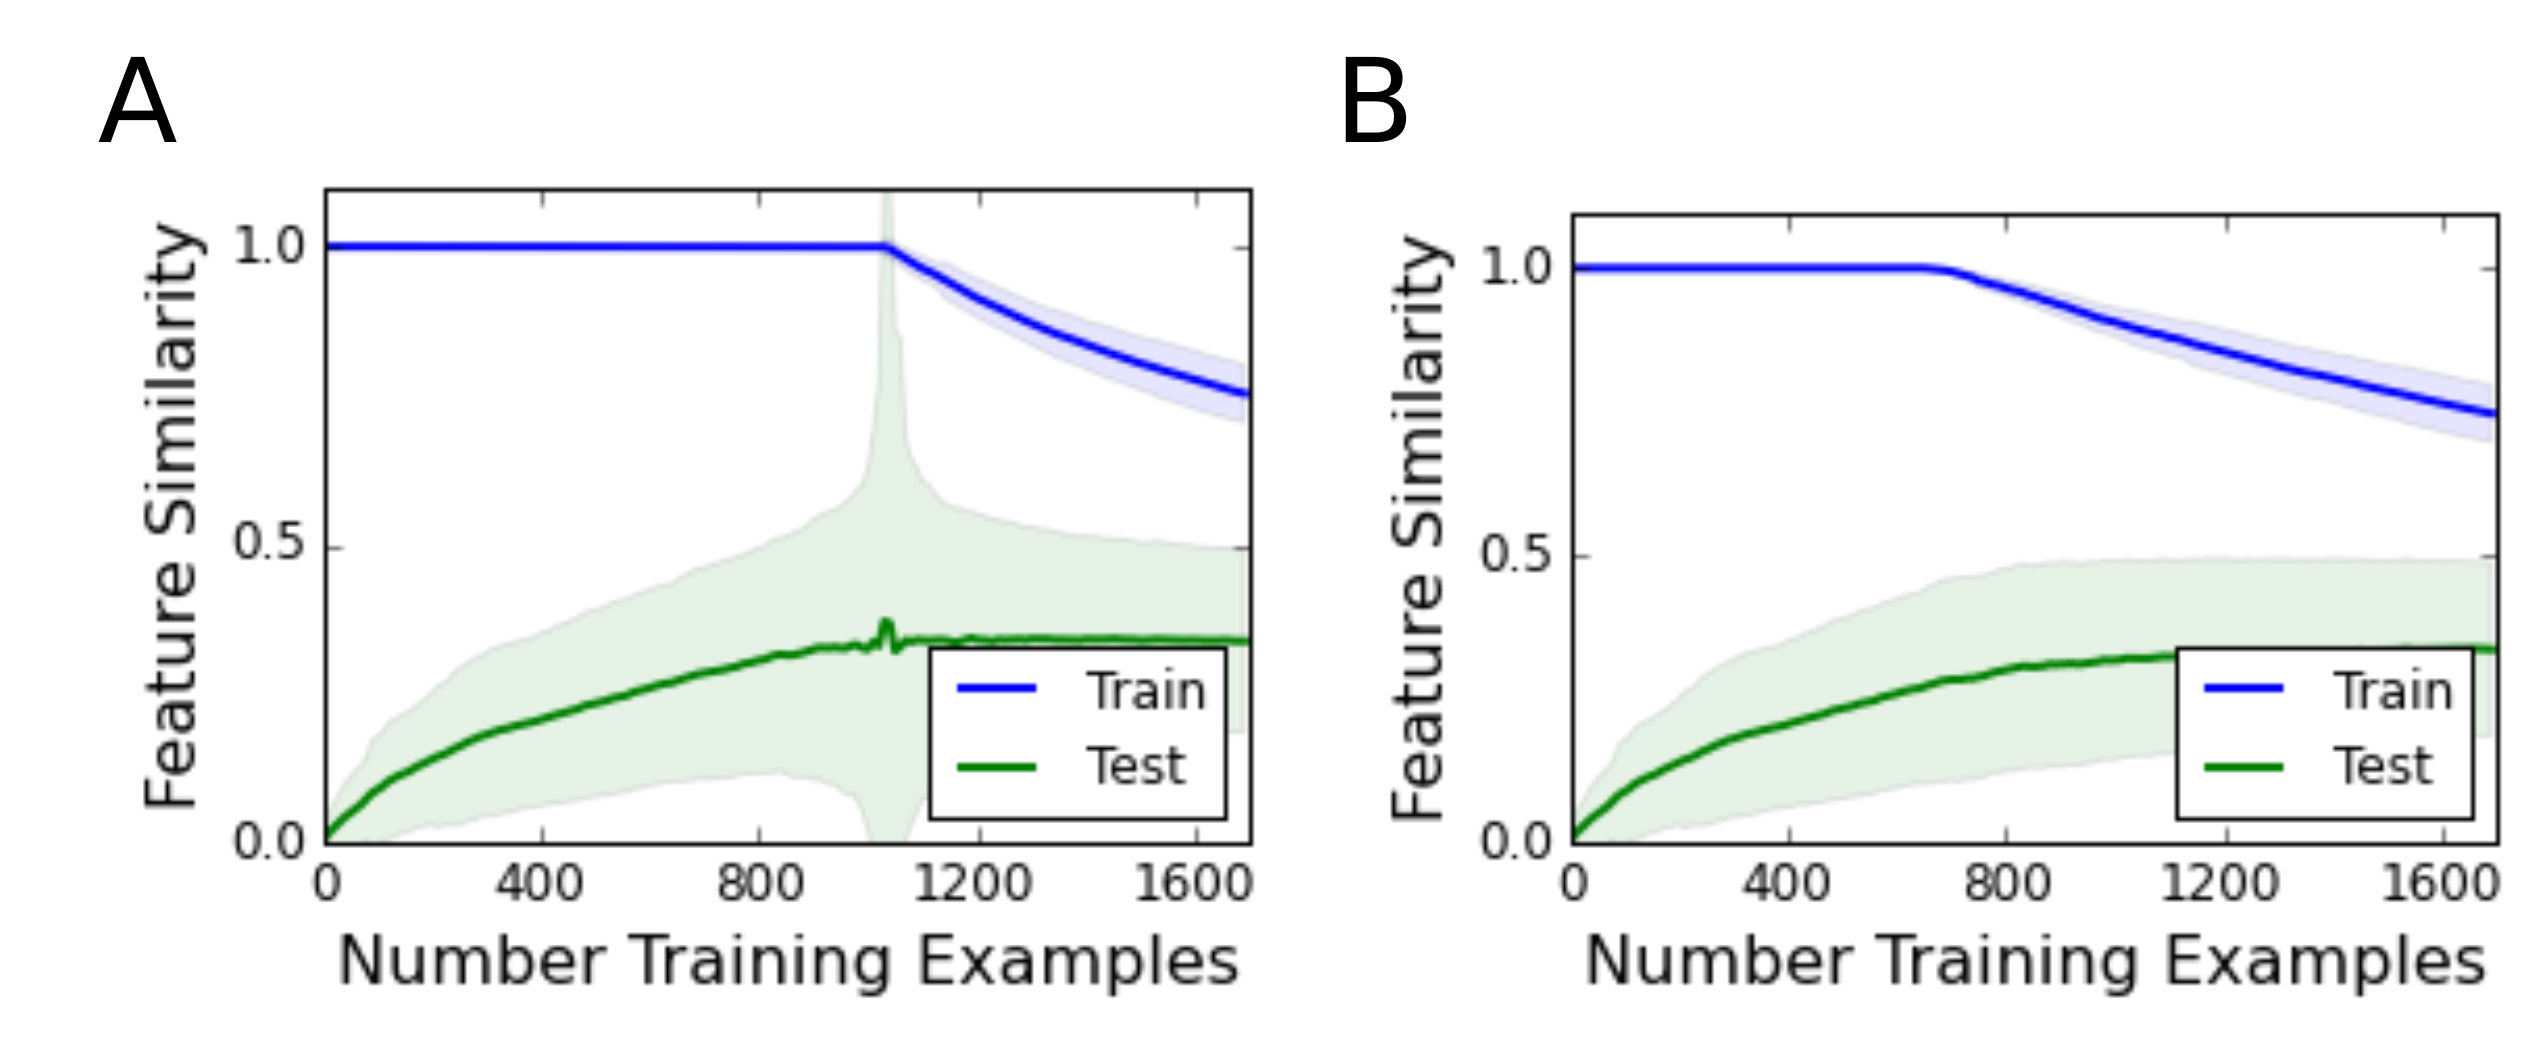
\includegraphics[width=0.6\textwidth]{regression_issue-170518.png}
\caption{\textbf{Regression overfitting and singular value cutoff}}
\end{figure}

The dictionary algorithm can be seen to generalize to the test set, but it is challenging to interpret its performance purely in the abstract feature space. We see that the training set similarity increases beyond the normal value, which indicates that the network is over-emphasizing some aspects of the transformation. Essentially, this increase beyond $N$ in similarity is due to the same force that allows the network to generalize to novel verbs. As more verb pairs are added to the dictionary, then the common transformations start to stand out and get emphasized. The verbs in the training set all contribute to the similarity of the output, and many of them are contributing the same thing -- namely the regular rule of adding the trigram "ed." to create the past tense verbs. This explains the similarity going above $N$, as many verb-pairs are shouting the same correct feature. 

\begin{figure}
\centering
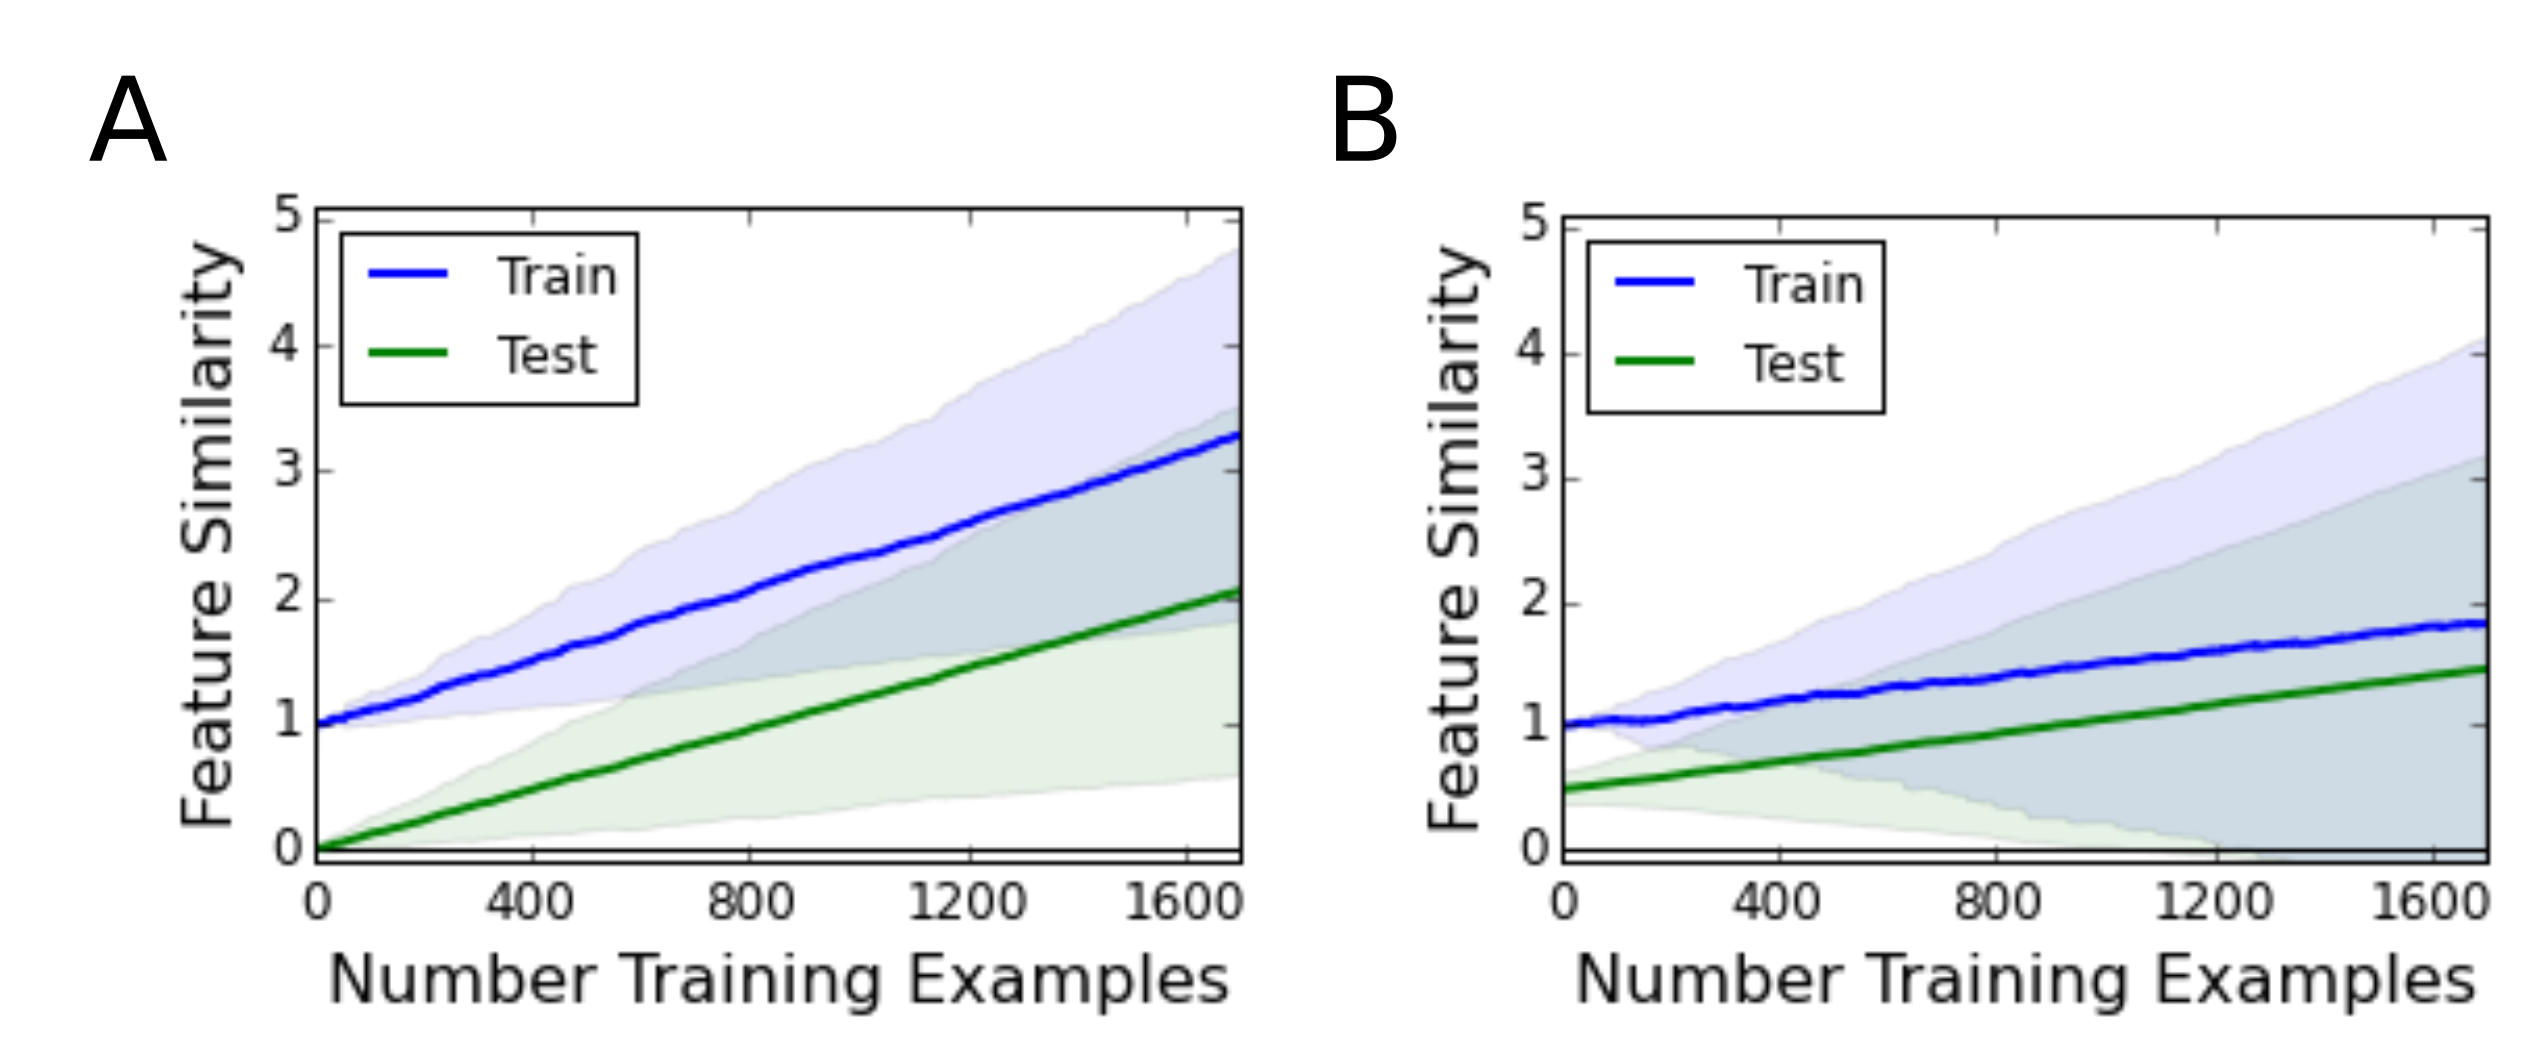
\includegraphics[width=0.6\textwidth]{dictionary_issue-170518.png}
\caption{\textbf{Hypercomputing dictionary issue with correlated inputs}}
\end{figure}

\section{Algorithms and Results}

\subsection{Matrix Algorithms}

The binding mechanism described for hypercomputing is a vector operation, but \citet{Rumelhart1986a} proposed matrices as the base unit for neural networks. A straight-forward approach to solve the transformation in matrix space is to perform a linear regression between present tense and the past tense hypervectors. The \emph{memory matrix} $\mathbf{W}$ is now an $N \times N$ matrix corresponding to the least squares solution. We use this as our baseline evaluation for learning transformations. We use linear regression as the optimal result of the online learning algorithm. Given that binding and unbinding and linear operations, we can interpret linear regression as a binding and optimal regularization. We interpret the online algorithm as an approximation to a closed form solution for learning grammatical rules. 
NOTE: If we interpret a regression model as a layer in a neural net, can we say that a benefit of knowing the state of the online algorithm would be to know why and how a hidden layer is constructed?

\begin{figure}
\centering
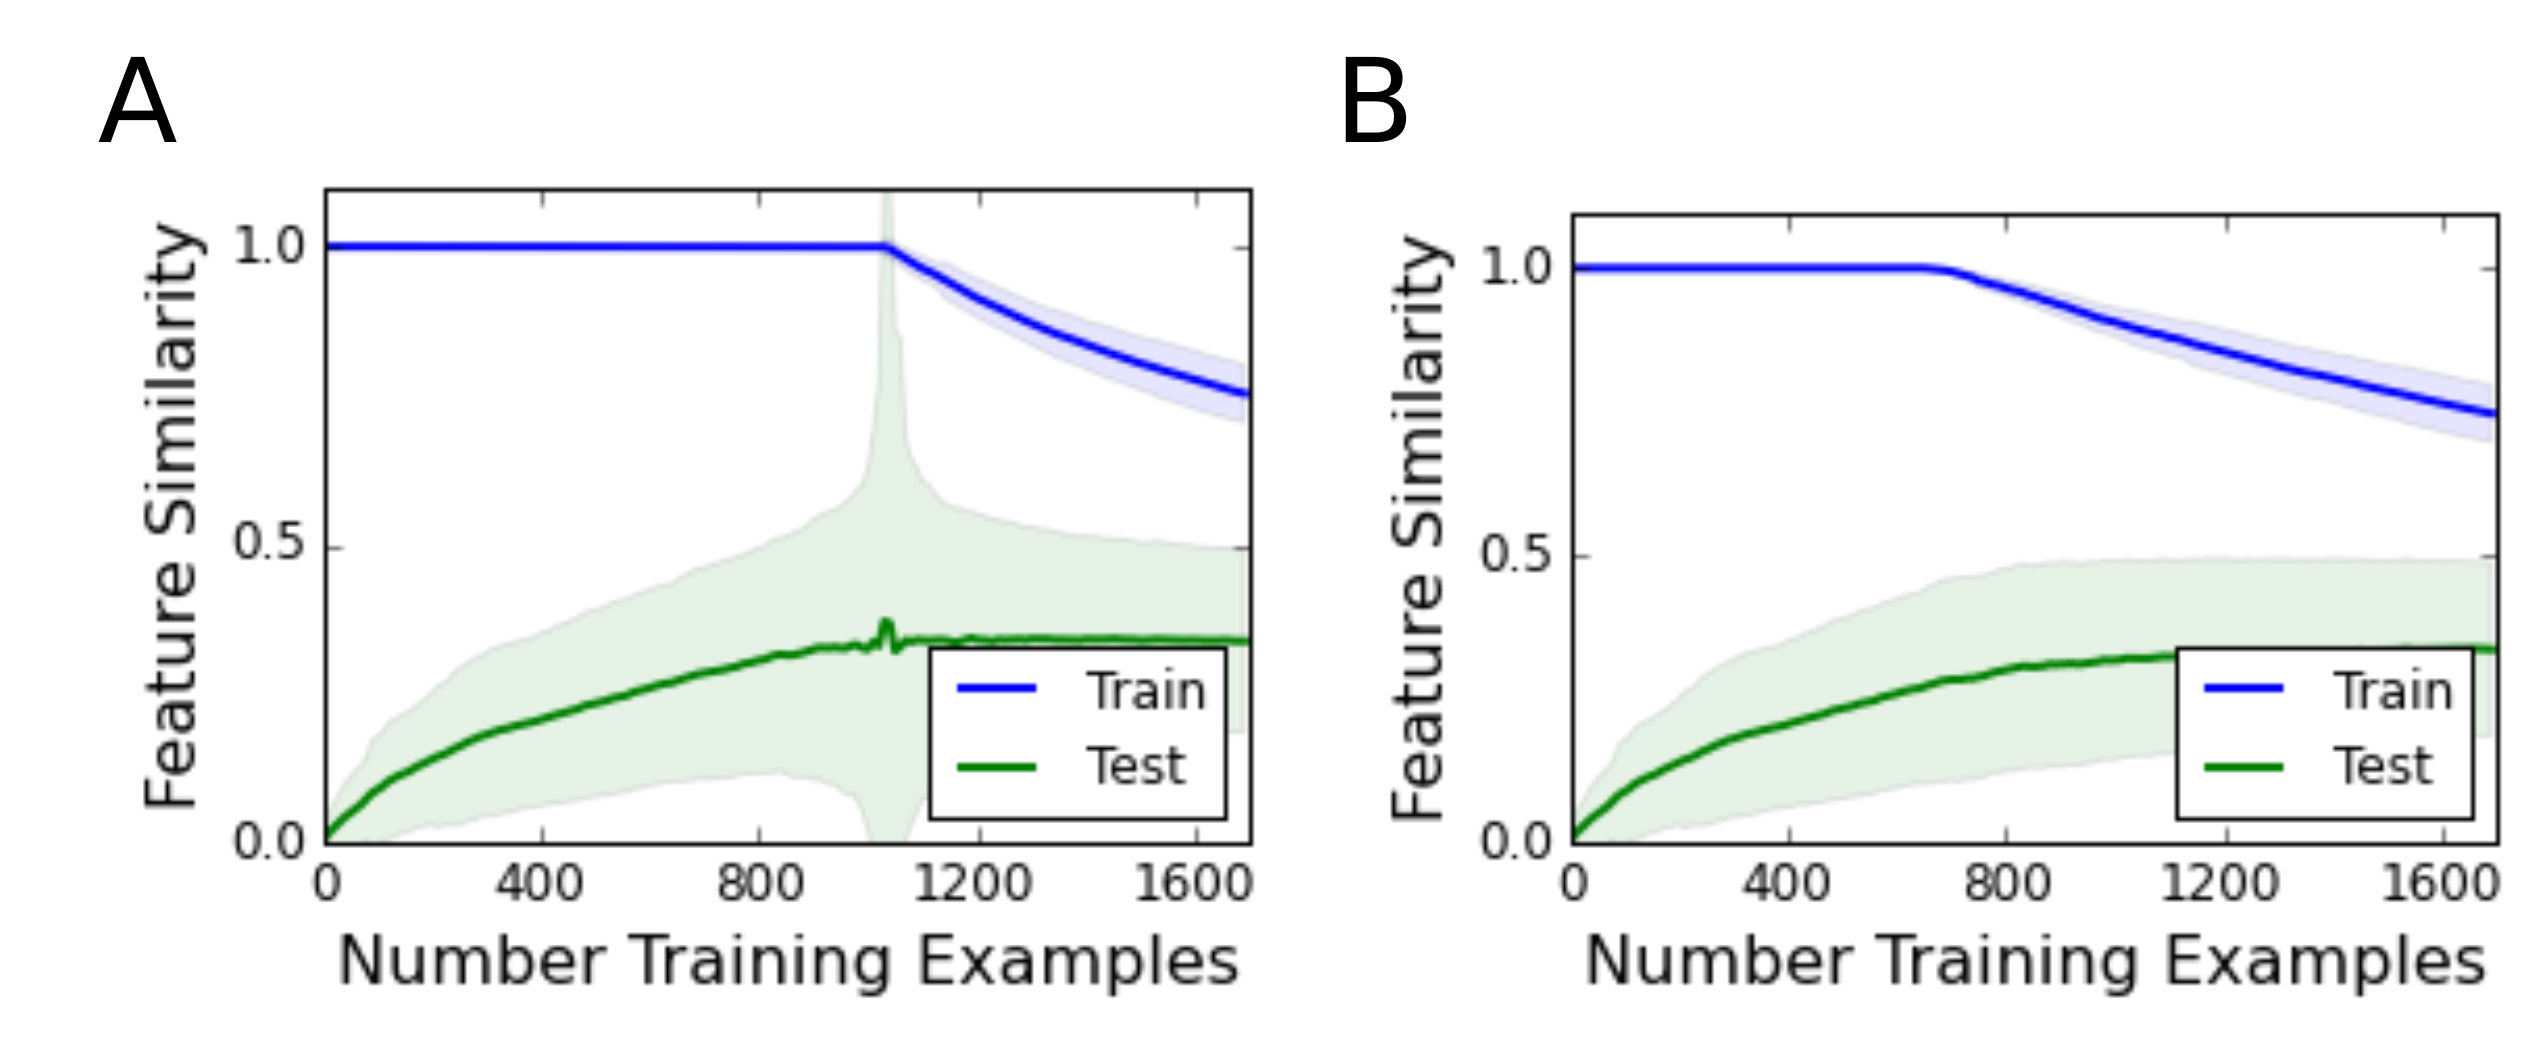
\includegraphics[width=0.6\textwidth]{regression_issue-170518.png}
\caption{\textbf{Least Squares solution for transforming hyper vectors.}}
\end{figure}

In the case of regression, all data must be available at compute time and requires computationally expensive matrix operations. Additionally, the singular values for the least squares solutions approaches really small numbers as the sample availability approaches $N$, resulting in an exploding similarity measure similar to an unregularized approach or overfitting. By setting a minimum singular value, we get a similar regularized learning rule. 
NOTE: We can take a closer look at the singular values to see why the model is not generalizing as much as it should. We can try to tune the singular values / the construction of singular values to emphasize patterns that represent grammatical rules instead of the status quo - emphasize the verb root.

We propose an approach to approximate online regression by defining an error and performing gradient descent step at each iteration, with the gradient step defined as:

\begin{equation}
\Delta \mathbf{W} = \alpha (\Psi^{past}_{v2} - \mathbf{W} \Psi^{present}_{v1}) \Psi^{present^\top}_{v1}
\end{equation}


\begin{figure}[h]
\centering
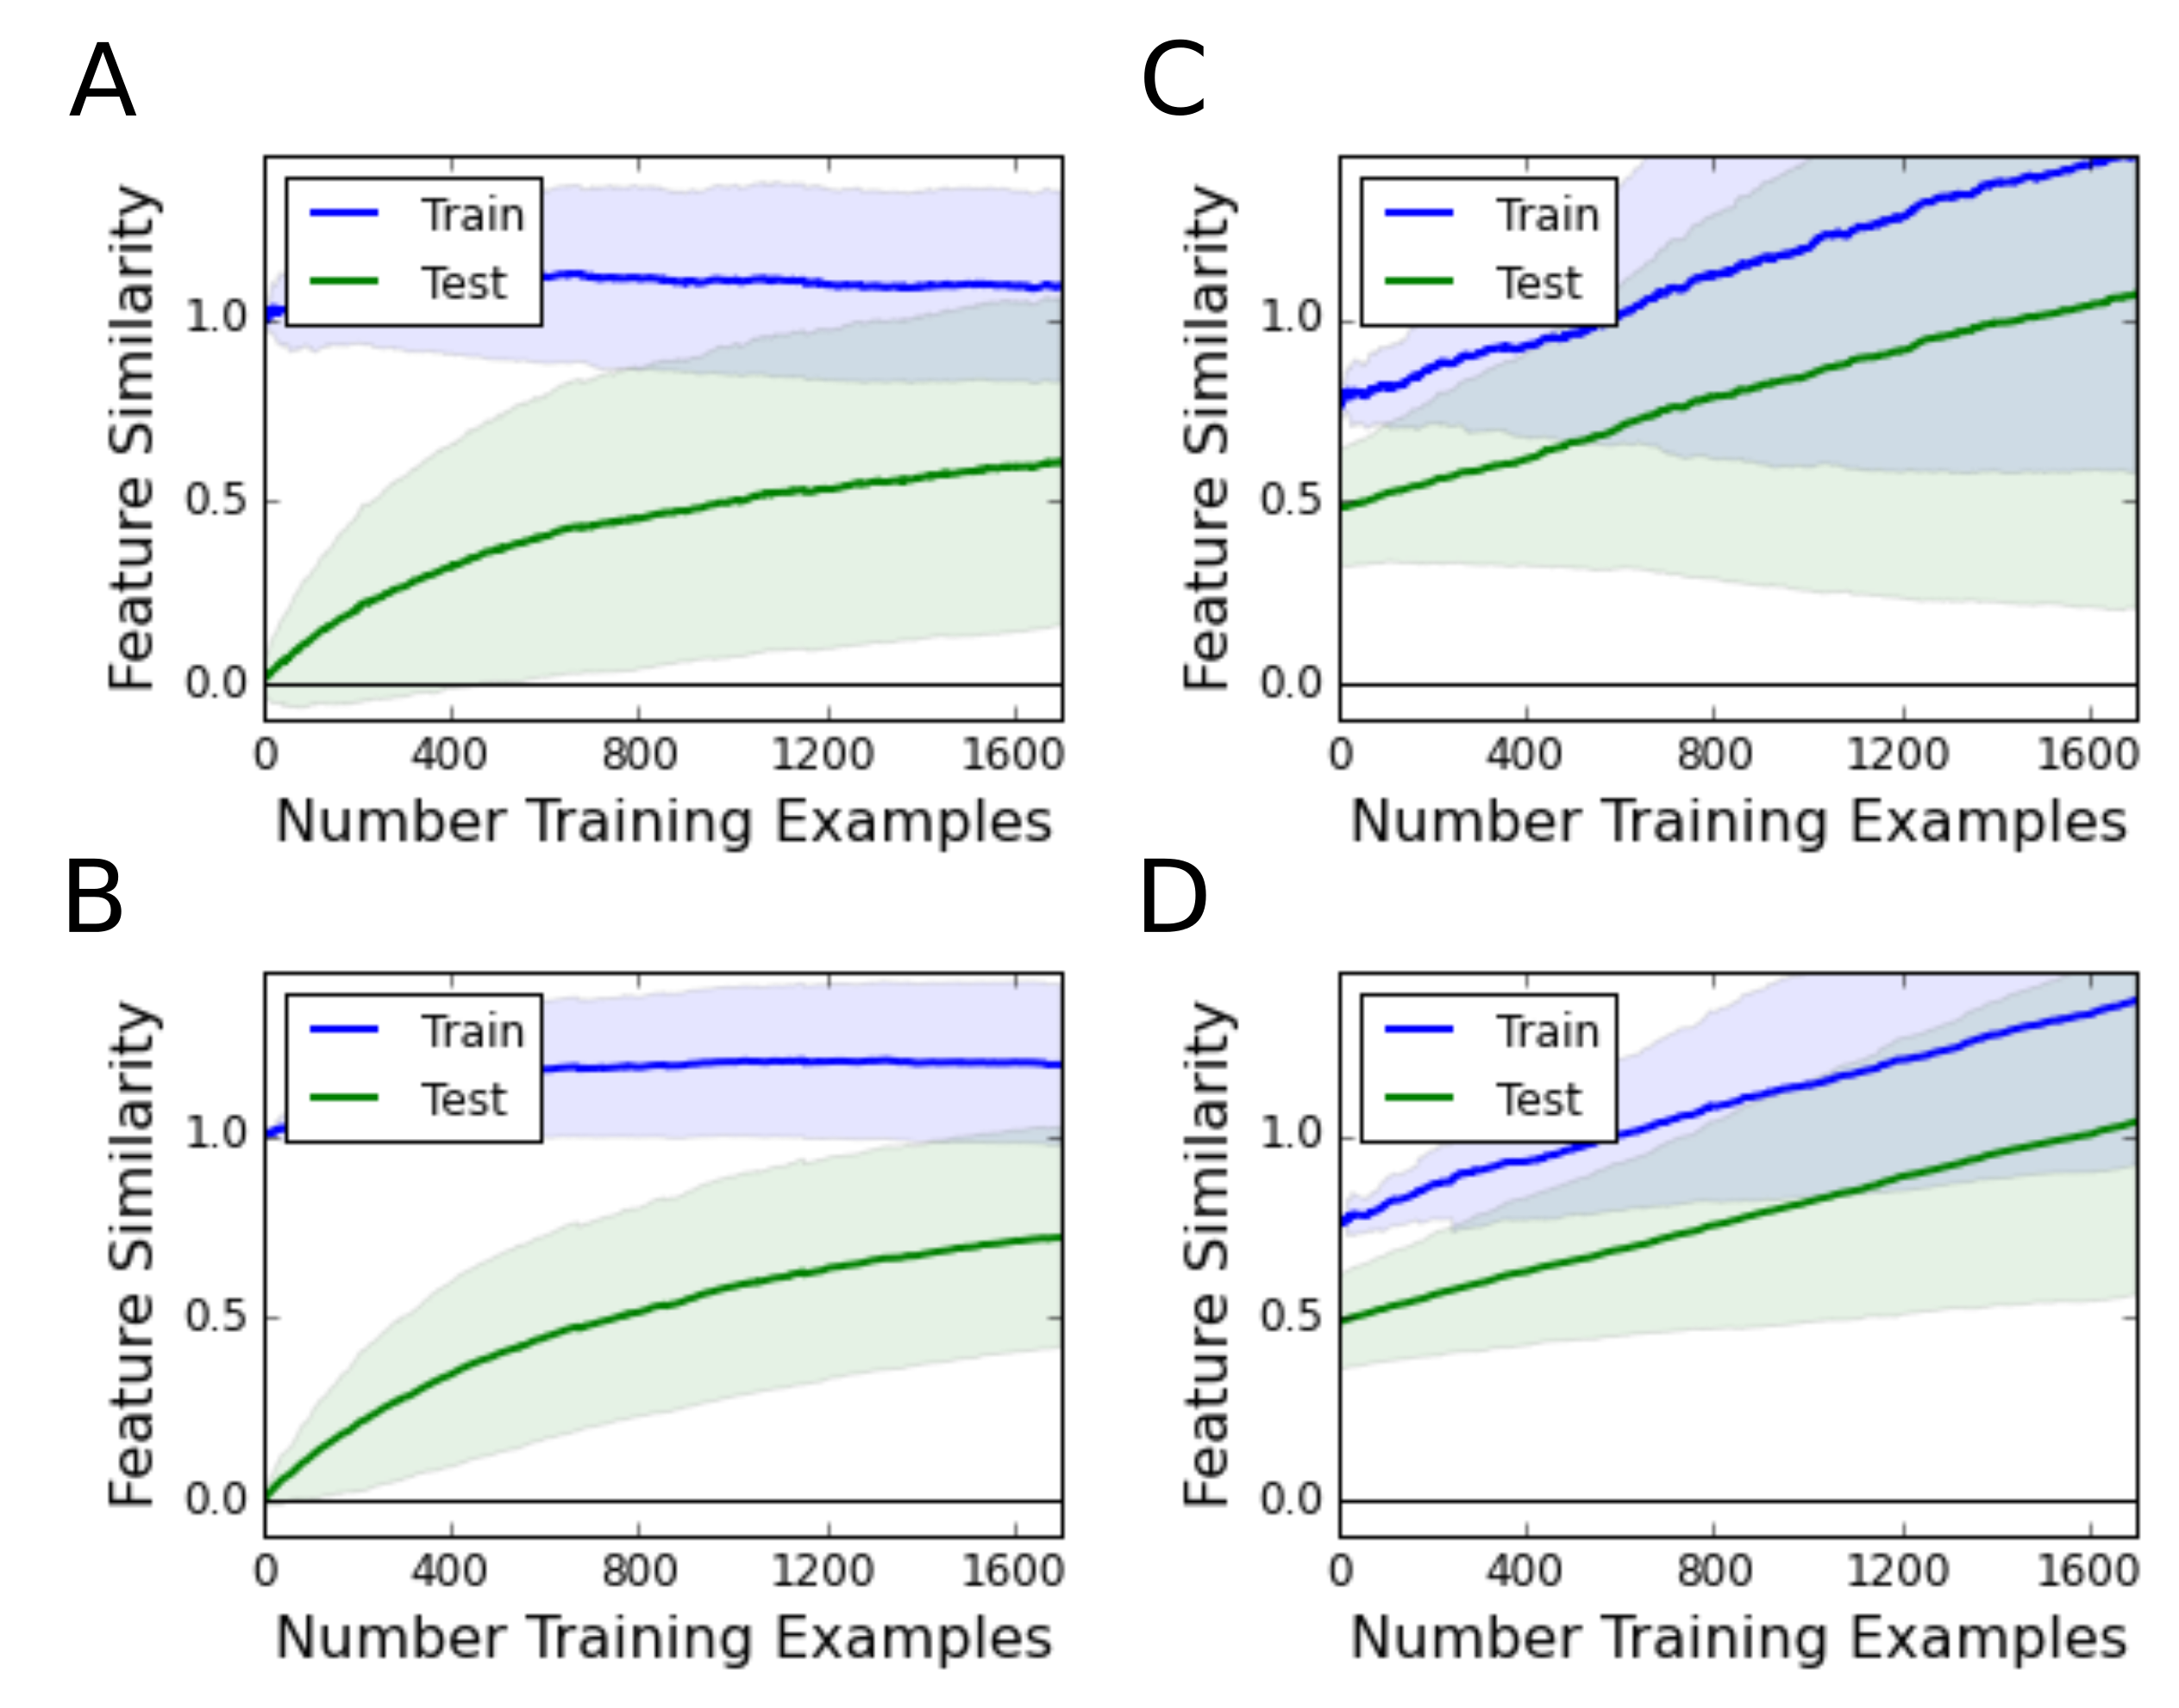
\includegraphics[width=0.6\textwidth]{outer_product_algorithm-170518.png}
\caption{\textbf{Matrix binding online algorithm}}
\end{figure}

A benefit of the matrix algorithm is the ability to add more vectors, since similarity measures only taper off, not decrease from regularization.

\begin{figure}[h]
\centering
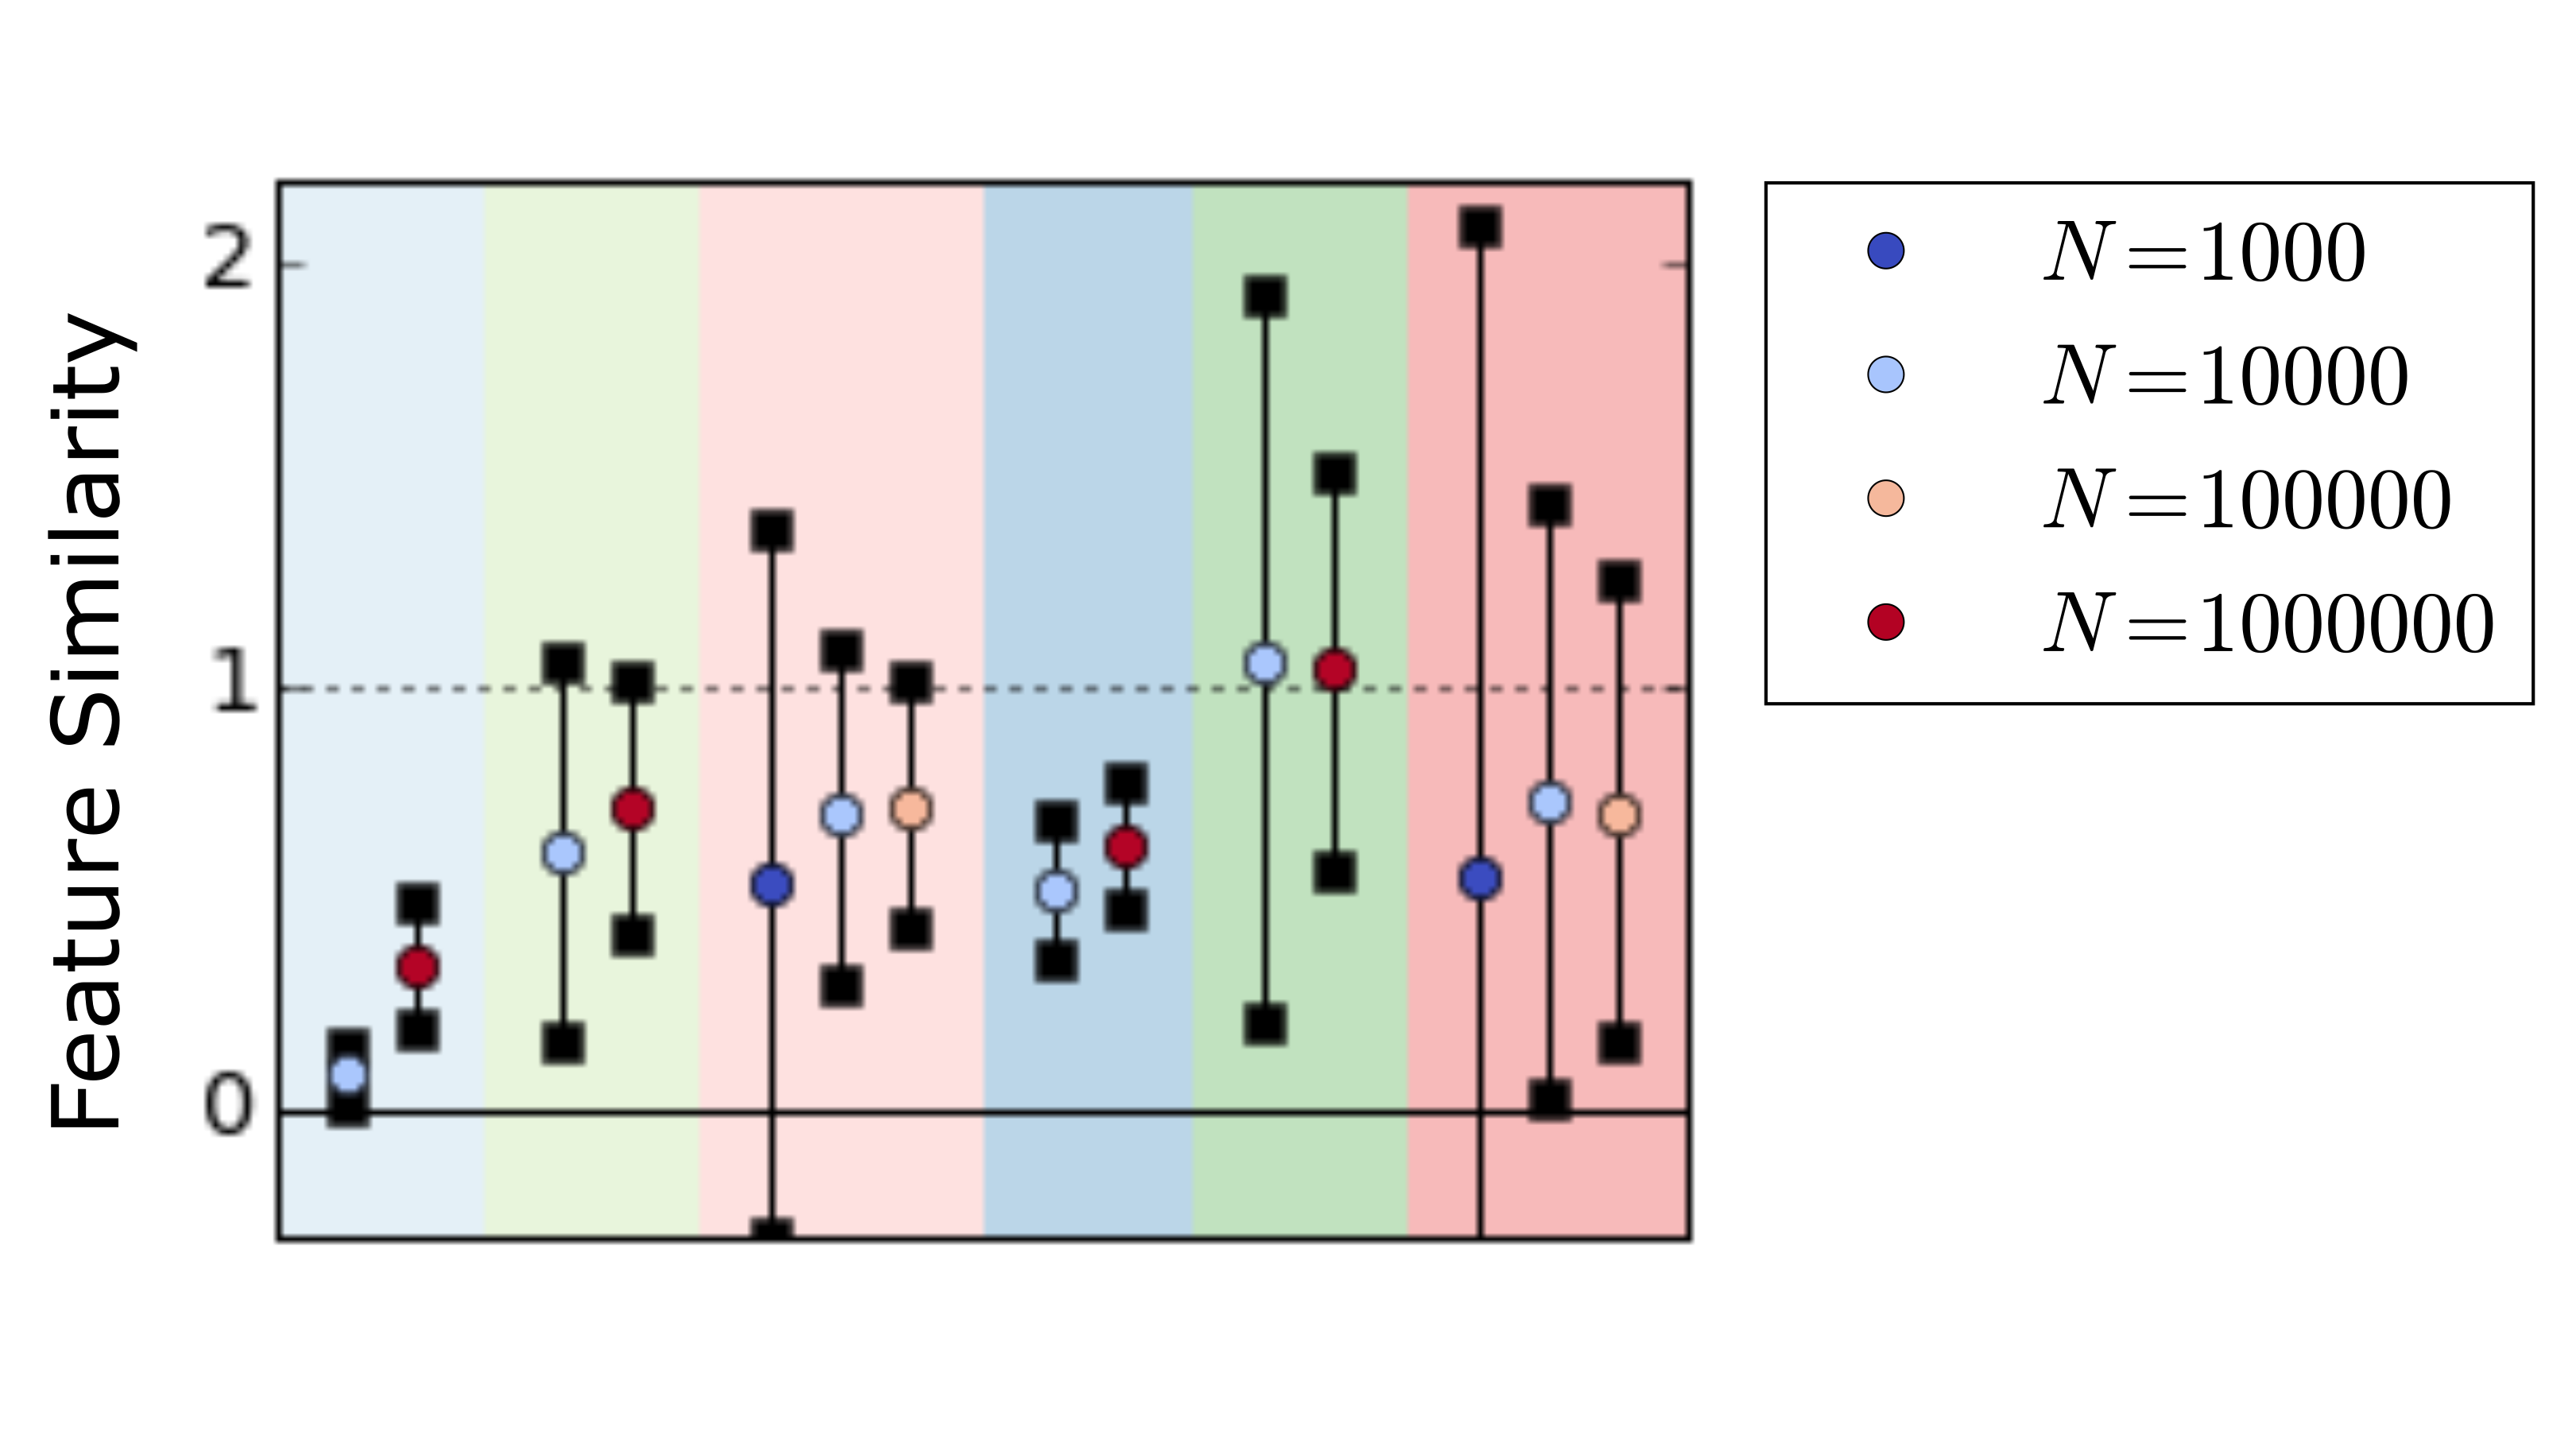
\includegraphics[width=0.6\textwidth]{algorithm_comparison-170519.png}
\caption{\textbf{Algorithm comparison} The test performance of the regression baseline (blue background) is compared to the performance of the matrix algorithms (green background) and the vector algorithms (red background). Colored circles indicate number of parameters in the network, $N=[10^3, 10^4, 10^5, 10^6]$. The vector algorithms outperform on test generalization than the regression, and have similar performance to the matrix algorihtm with fewer parameters.}
\end{figure}

\subsection{Vector Algorithms}

The naive hypervector framework presented above serves as the foundation for our learning algorithms. The above learning rule is considered unregularized because at any given update-step, the weight of the incoming word is added regardless of the current memory vector's state. Since the memory vector tries to capture every information presented, the same structural features are repeatedly summed together resulting in an unbounded similarity metric.

The resulting similarity can be interpreted as the amount of underlying structure. Similarity associated with highly organized transformations increase quickly because many of the common features are re-emphasized repeatedly. Figure 1A  uses the regular binding and shows that hypervector mappings are unsurprisingly highly organized. Figure 1B shows that the difference binding removes many of the redundant trigrams, decreasing the similarity but allowing the model to capture more nuances.

For learning this isn't particularly useful because similarity can be arbitrarily large. In order to prevent an arbitrarily large memory vector, we use a regularization procedure that evaluates the error of a new word in the training set prior to adding it to our working memory $\Omega$. More specifically, the new word vector is scaled by how dissimilar the dereferenced prediction is to the true hypervector.

\begin{align}
\label{eq:regularization_vec}
\notag \alpha &= \frac{N-\Psi^{past\top}_{v2} \Omega \circ \Psi^{present}_{v1}}{N}  \\
\Omega_n &= \Omega_{n-1} + \alpha \Psi^{present}_{v1} \circ \Psi^{past}_{v2}
\end{align}

\begin{align}
\label{eq:regularization_difference_vec}
\notag \alpha &= \frac{N-
\Psi^{past\top}_{v2} (\Psi^{present}_{v1} \circ \Omega+
\Psi^{past}_{v1})}{N} \\
\Omega_n &= \Omega_{n-1} + \alpha
(\Psi^{past}_{v2} - \Psi^{present}_{v2})
\Psi^{present}_{v1}
\end{align}

By first measuring how strongly other words in the training set predict the transformation of the new verb-pair, we have an update rule that avoids saturating the memory vector with common transformation. With this regularization rule, we now can see a network that one-shot memorizes the training set accurately and can still generalize on unseen examples. Furthermore we see that the difference binding can spend more of it's bits focusing on the non-trivial transformation parts, allowing it to achieve slightly better results.


\begin{figure}[h]
\centering
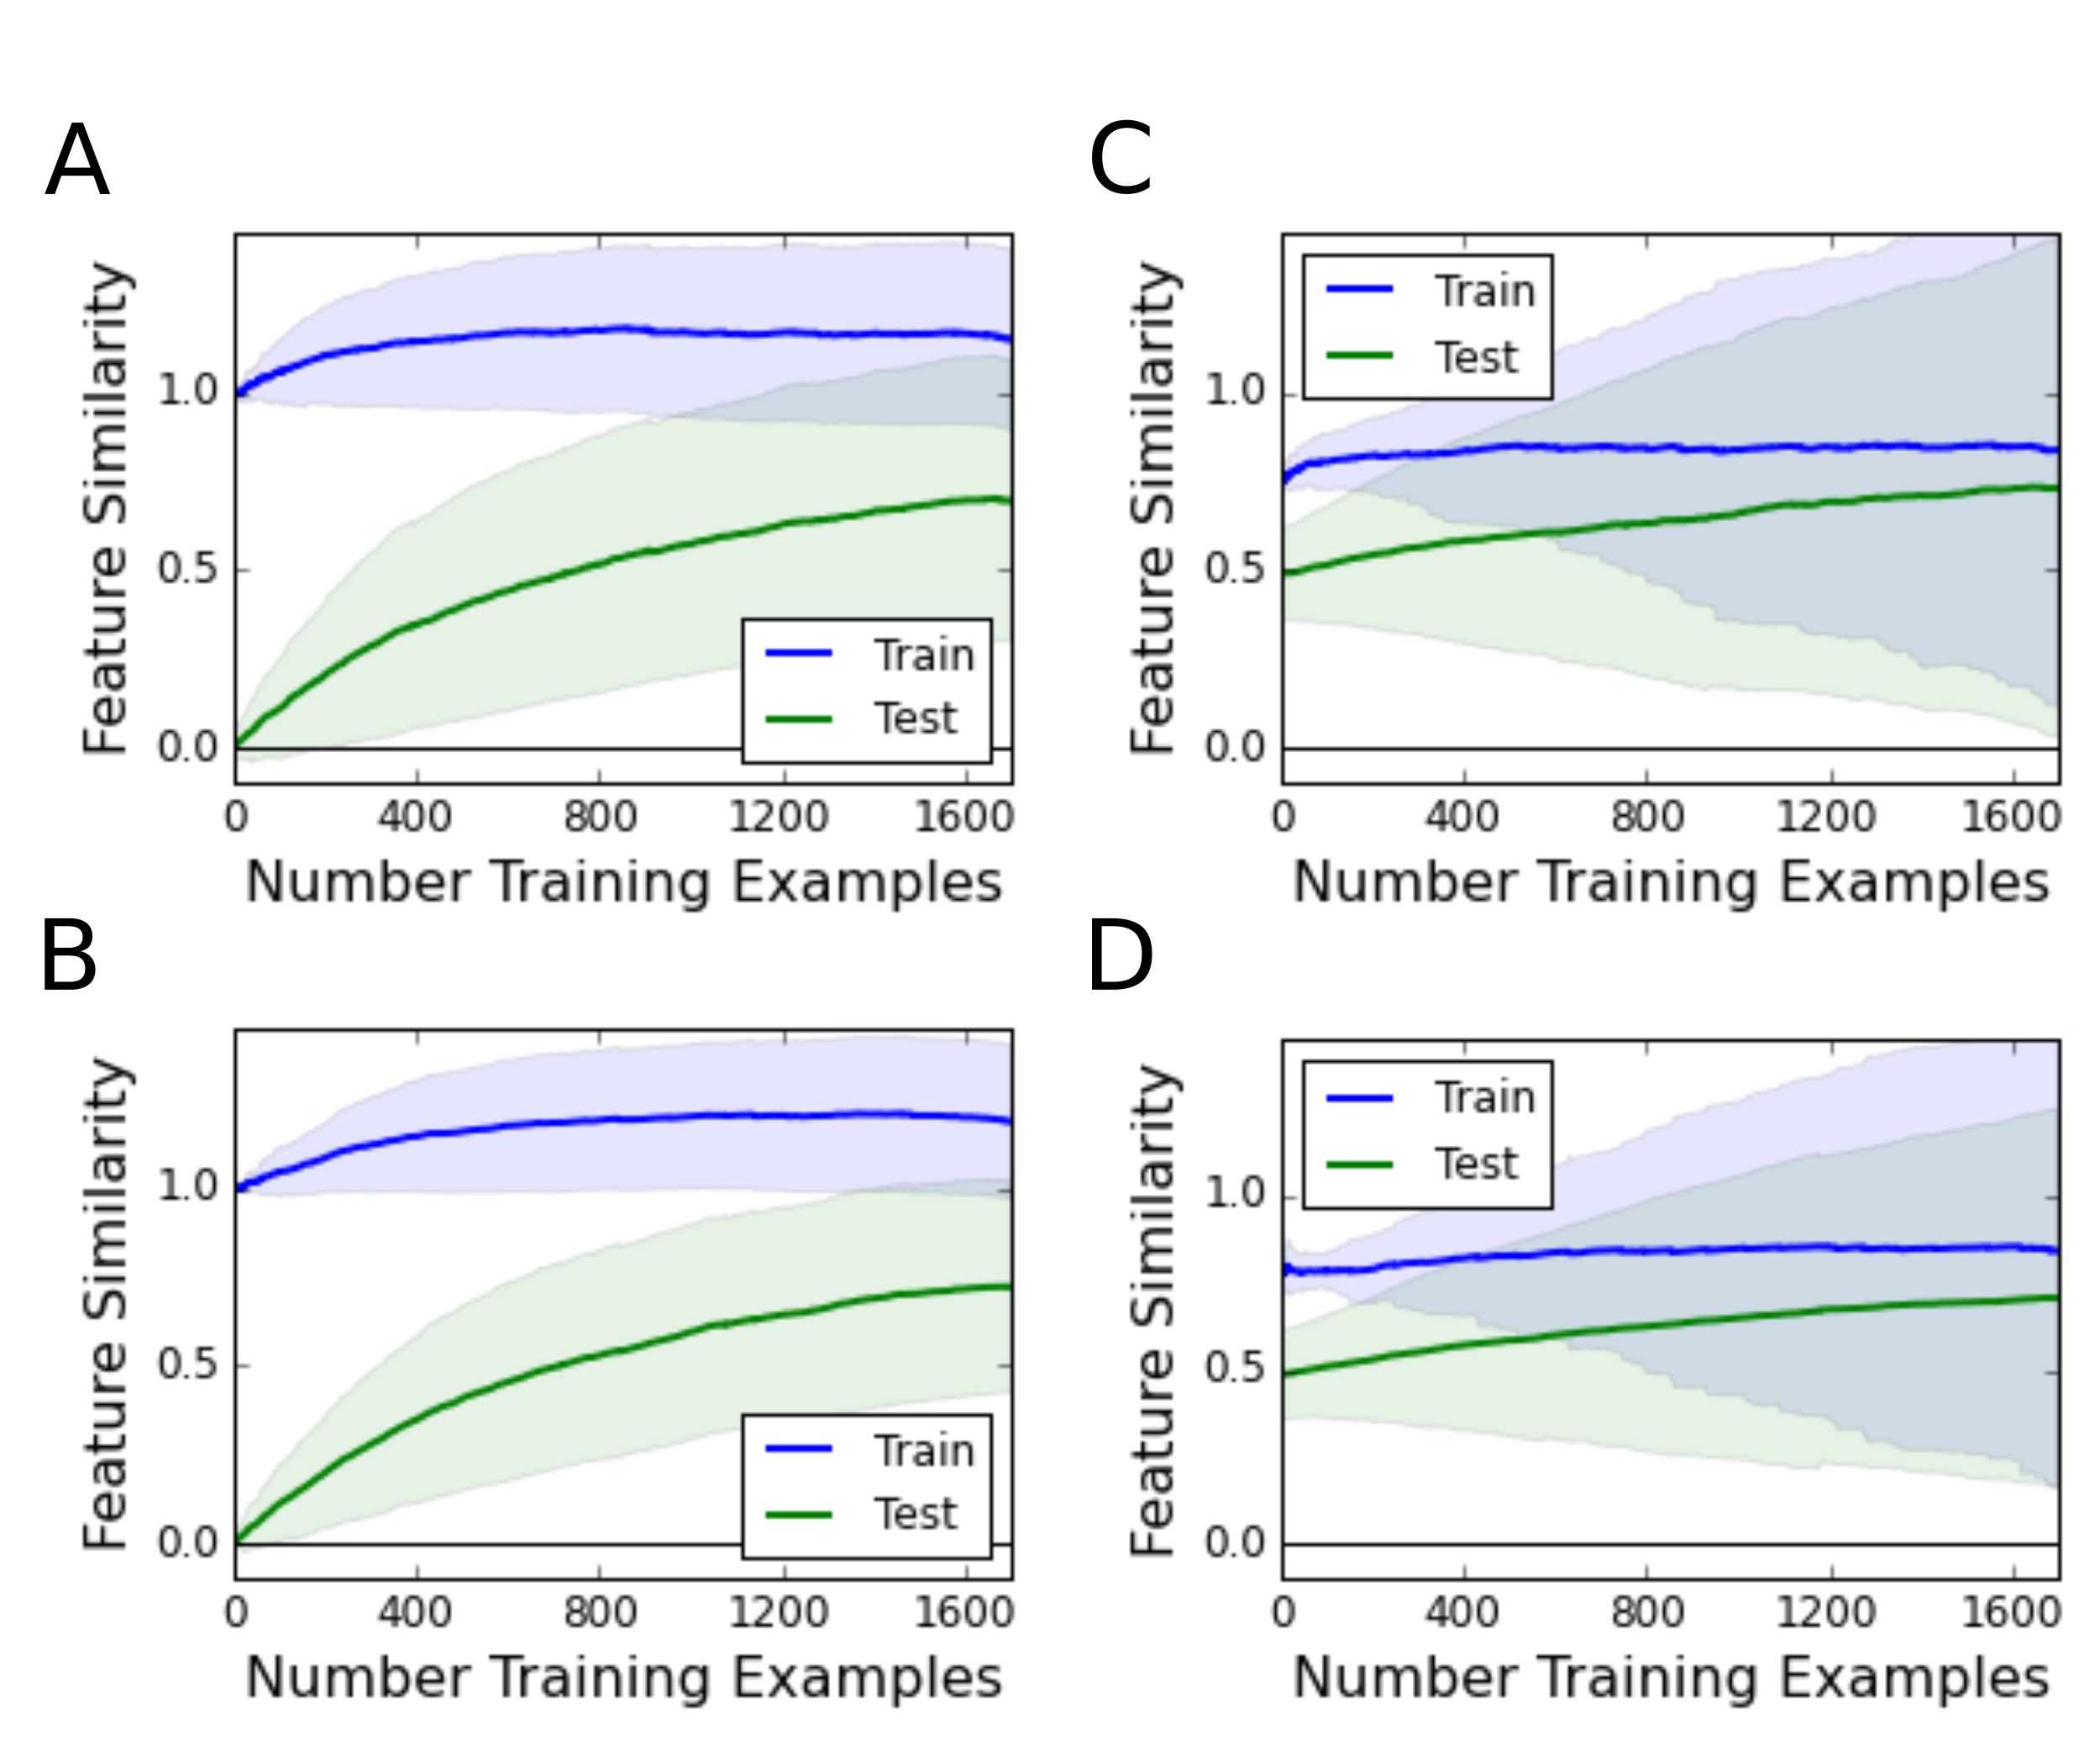
\includegraphics[width=0.6\textwidth]{vector_binding_algorithm-170518.png}
\caption{\textbf{Vector binding online algorithm.} A. Unregularized binding. B. Unregularized difference binding. C. Regularized binding. D. Regularized difference binding.}
\end{figure}

The new update rule bounds the similarity measure to 1, which means that the maximum measure of similarity is satisfied when two vectors are identical. Similarity measures aren't as deceiving by filtering out the noise other inputs contribute to the model. Train and test error are now closer. The difference vector algorithm performs better by explicitly binding only the sequence of letters that compose the past tense of a verb to the present tense of the same verb. 


\section{Discussion}
The regression solution can be better understood through connection to hyperdimensional computing and the binding mechanism. The original proposals for binding \citet{Smolensky1990} required formation of the outer product between the two input vectors. However, this was a problem for many computational frameworks due to the need to explode the state-space by forming higher and higher order tensor products to create bound structures. \citet{Plate1991} described a new type of binding mechanism, \emph{circular convolution}, which could be used in place of the outer-product rule but also maintained the dimensionality of the two input vectors. Plate noted that circular convolution acts as a compressed outer product. The binding mechanism used in hyperdimensional computing ($\times$, element-wise multiplication) and in general can also be described as the compressed outer product. 

NOTE: To further explain why our binding is related to circular convolution: We can describe construction of a word as the nested convolution between letter functions. Another reason why this is preferable to outer product is because the outer product captures all of the relationships between letters that isn't exactly necessary. Can we say this is similar to holding the entire covariance matrix of a set of letter vectors? In other words, although there is more space, in fact, $O(n^2)$ more space to store information, more of the space is used. Circular convolution preserves the relationships between letters, or the signal a word would make enough to differentiate between other word vectors and emphasizes similar ngram patterns.


Through the connection of binding, outer-products and matrix multiplication, we can now see that there is a simple regularization procedure that gradient descent utilizes. This can allow us to combine the dictionary one-shot learning techniques of hyperdimensional computing with the ability to generalize a high-level feature space.
NOTE: High-level feature spaces are valuable because they are explicit semantic vectors that can be "spelled out" by more mechanical features. We can probably now have "king" = "queen" - "man" with simpler operations, maybe even literal subtractions rather than relying on a series of non-linear operations that would indirectly compute the subtraction. We also (can I say this?) don't have to rely on defining a unique vector to represent each meaning or enumerate rather than computing meanings via vectors. 

CITE:
https://arxiv.org/abs/1509.01692
http://aclweb.org/anthology/C16-1332


Further cycles through the training data can solidify the verb pairs in the training set in the dictionary. This could also be helpful for generalization, but it is hard to tell if performance in the test set improved with the second cycle.  This regularized form of the algorithm can also iterate through the training data more than once. If we show it all of the training words a second time, we can improve its performance.

NOTE: Given the amount of noise in the dereferenced vector/prediction, we should refine the prediction with Paxon's resonance attractor. Then measure this refined prediction against the ground-truth vector. Currently, the resonance attractor doesn't generalize enough or places too much weight on the not tense specific part of the word (which is why we're trying the difference algorithm) that 

\section{Conclusion}
We have shown that hypervector algorithms provide a way for learning transformations in data in an online and one-shot manner. While the output of the transformations still operate in hypervector space, there exist ways to recover the original data when computing at sufficiently high $N$. 

A potential method is the resonance attractor, which at sufficiently high N can recall a noisy representation and refine it to most closely match to its ground truth. It currently is not able to generalize because when a prediction is refined, each state of the prediction refers its previous state- which makes sense for denoising, but not for extrapolating. 
NOTE: More working is currently being done for generalization. 

Our other contribution is within the realm of Parallel Distributed Processing and how the greater literature fits in with neural networks. While the optimization behavior for neural networks are not well known, our work demonstrates that a high-dimensional encoding of features and linear binding transformations can capture similar behavior as low-dimensional non-linear functions. Non linear functions, in other words, hidden layers in a neural net, can have their results be mirrored and explained by linear transformations in high enough dimensions. In the worst case, linear transformations are paired with simple, non-linear functions such as clipping. 
% There is a lot more to say about this so links will be attached.
% http://web.stanford.edu/~jlmcc/papers/PDP/Volume%201/Chap2_PDP86.pdf



% (Andrew): Anything below here I moved to the google docs:
% https://docs.google.com/document/d/1PUiixSRlxmuiTpZ6YzCuW75ibo0hlQbwalmxq26Wmh0/edit
% http://lolita.unice.fr/~scheer/cogsci/Rumelhart,%20McClelland%20et%20al%2086%20(Vol.1)%20-%20Parallel%20Distributed%20Processing-%20Exploration%20in%20the%20Micro-Structure%20of%20Cognition.pdf
% https://academiaanalitica.files.wordpress.com/2016/11/david-e-rumelhart-james-l-mcclelland-pdp-research-group-parallel-distributed-processing_-explorations-in-the-microstructure-of-cognition_-foundations-vol-11986.pdf
% http://users.ecs.soton.ac.uk/harnad/Papers/Py104/pinker.conn.html
% https://www.research.manchester.ac.uk/portal/files/54562944/FULL_TEXT.PDF
% http://web.stanford.edu/~jlmcc/papers/PDP/Volume%201/Chap1_Part1_PDP86.pdf
% https://stanford.edu/~jlmcc/papers/PDP/Chapter1.pdf
% http://onlinelibrary.wiley.com/store/10.1111/cogs.12148/asset/cogs12148.pdf;jsessionid=F76849F5198C92223DA660BAB456746F.f03t02?v=1&t=j68gehm4&s=f76e794c9dfa3e1e31898a881d7ddc89379f7500&systemMessage=Wiley+Online+Library+will+be+unavailable+on+Saturday+12th+August+at+3%3A00+EDT+%2F+8%3A00+BST+%2F+12%3A30+IST+%2F+15%3A00+SGT+for+4+hours+for+essential+maintenance.+Apologies+for+the+inconvenience.
% http://cseweb.ucsd.edu/~gary/PAPER-SUGGESTIONS/Jordan-TR-8604.pdf
% https://www.research.manchester.ac.uk/portal/files/54562944/FULL_TEXT.PDF


%\subsubsection*{Acknowledgments}
%


\bibliographystyle{abbrvnat}
%\bibliographystyle{abbrv}
\bibliography{hdprespast}

% [1] Alexander, J.A.\ \& Mozer, M.C.\ (1995) Template-based algorithms
% for connectionist rule extraction. In G.\ Tesauro, D.S.\ Touretzky and
% T.K.\ Leen (eds.), {\it Advances in Neural Information Processing
%   Systems 7}, pp.\ 609--616. Cambridge, MA: MIT Press.

% [2] Bower, J.M.\ \& Beeman, D.\ (1995) {\it The Book of GENESIS:
%   Exploring Realistic Neural Models with the GEneral NEural SImulation
%   System.}  New York: TELOS/Springer--Verlag.

% [3] Hasselmo, M.E., Schnell, E.\ \& Barkai, E.\ (1995) Dynamics of
% learning and recall at excitatory recurrent synapses and cholinergic
% modulation in rat hippocampal region CA3. {\it Journal of
%   Neuroscience} {\bf 15}(7):5249-5262.

\end{document}